\chapter{Materiais e Métodos}

Esta seção descreve as etapas do desenvolvimento da API, assim como a aplicação e utilização das ferramentas e suas tecnologias. Este desenvolvimento foi realizado utilizando a generalização de conceitos de engenharia de software, com o objetivo de um baixo acoplamento e alta coesão assim também como a reutilização de código. As etapas de desenvolvimento se deram através dos estágios necessários para a construção de uma API REST e foram organizadas utilizando a metodologia ágil Kanban.

\section{Bibliotecas e Ferramentas}

A escolha das bibliotecas e softwares deste projeto, devem-se a pesquisas que tiveram como foco: 
\begin{itemize}
    \item Suporte dos desenvolvedores: Dada a necessidade de se ter uma ferramenta que seja confiável e atualizada;
    \item Alta utilização pela comunidade: Já que a maioria destas ferramentas são de código livre e podendo a comunidade submeter melhorias e realizar a revisão do código que está sendo alterado na mesma;
    \item Compatibilidade a outros componentes e estrutura do projeto: Um dos objetivos deste software é que ele seja mutável, para que de acordo com as mudanças que podem ocorrer em outras tecnologias e estruturas de documentos PDF, esteja apto a acompanhar tais alterações.
\end{itemize}

\subsection{PDF.JS - v2.2.228}

O PDF.JS, criado em 2011 pela Mozilla Foundation, é uma biblioteca amplamente utilizada, e se encontra presente na maioria dos websites que fazem qualquer tipo de manipulação e exibição de PDF. Esta foi criada como uma extensão do navegador Firefox, com a intenção de renderizar arquivos PDF, de forma rápida e segura, no navegador do cliente. Apesar da migração de uma biblioteca específica para o navegador da Mozilla, seu formato de renderização permanece o mesmo, onde ela acessa a estrutura do arquivo PDF, coleta o conteúdo e a formatação no \textit{Body}, realiza a conversão para HTML e CSS de cada objeto encontrado e com a tabela XREF o arquivo é remontado no navegador do cliente como um PDF dentro da página web.

Com a evolução das tecnologias e a busca contínua por melhor performance, esta biblioteca conta com centenas de funções e diferentes abordagens para e leitura das mais variadas formas de PDF. Utilizando o resultado destas funções, é possível realizar extrações para coleta de informações encontradas no arquivo, informações como o texto puro, posição de elementos na página, fonte utilizada, cor e vários outros tipos.

Como o objetivo deste sistema está diretamente ligado a extração dos dados e o foco principal desta biblioteca é a renderização do arquivo no navegador, boa parte das funções mais pesadas nesta biblioteca não são necessárias.

\subsection{Extract - v0.1.3}
Convenientemente, há um módulo criado pela comunidade que encapsula somente a parte e extração de dados contida na biblioteca e entrega de forma leve e prática todas as funcionalidades necessárias para uma boa extração do conteúdo do arquivo PDF.

Fundamentalmente, a leitura acontece de forma que, dado o caminho do arquivo e um objeto de opções, são extraídos metadados do arquivo como o autor, o software utilizado para salvar o arquivo, o software utilizado para gerar o PDF, última data de edição entre outros. Junto ao objeto de metadados é retornado um vetor contendo um objeto JSON para cada página analisada, este objeto contém todas as informações básicas necessária para análise do conteúdo como é possível ver  \textbf{Figura \ref{pdfExtract}}.

\begin{figure}[H]
\centering
\captionsetup{justification   = raggedright,
              singlelinecheck = false}
\caption{Objeto JSON após extração de informação de um PDF através da biblioteca Extract.}\label{pdfExtract}
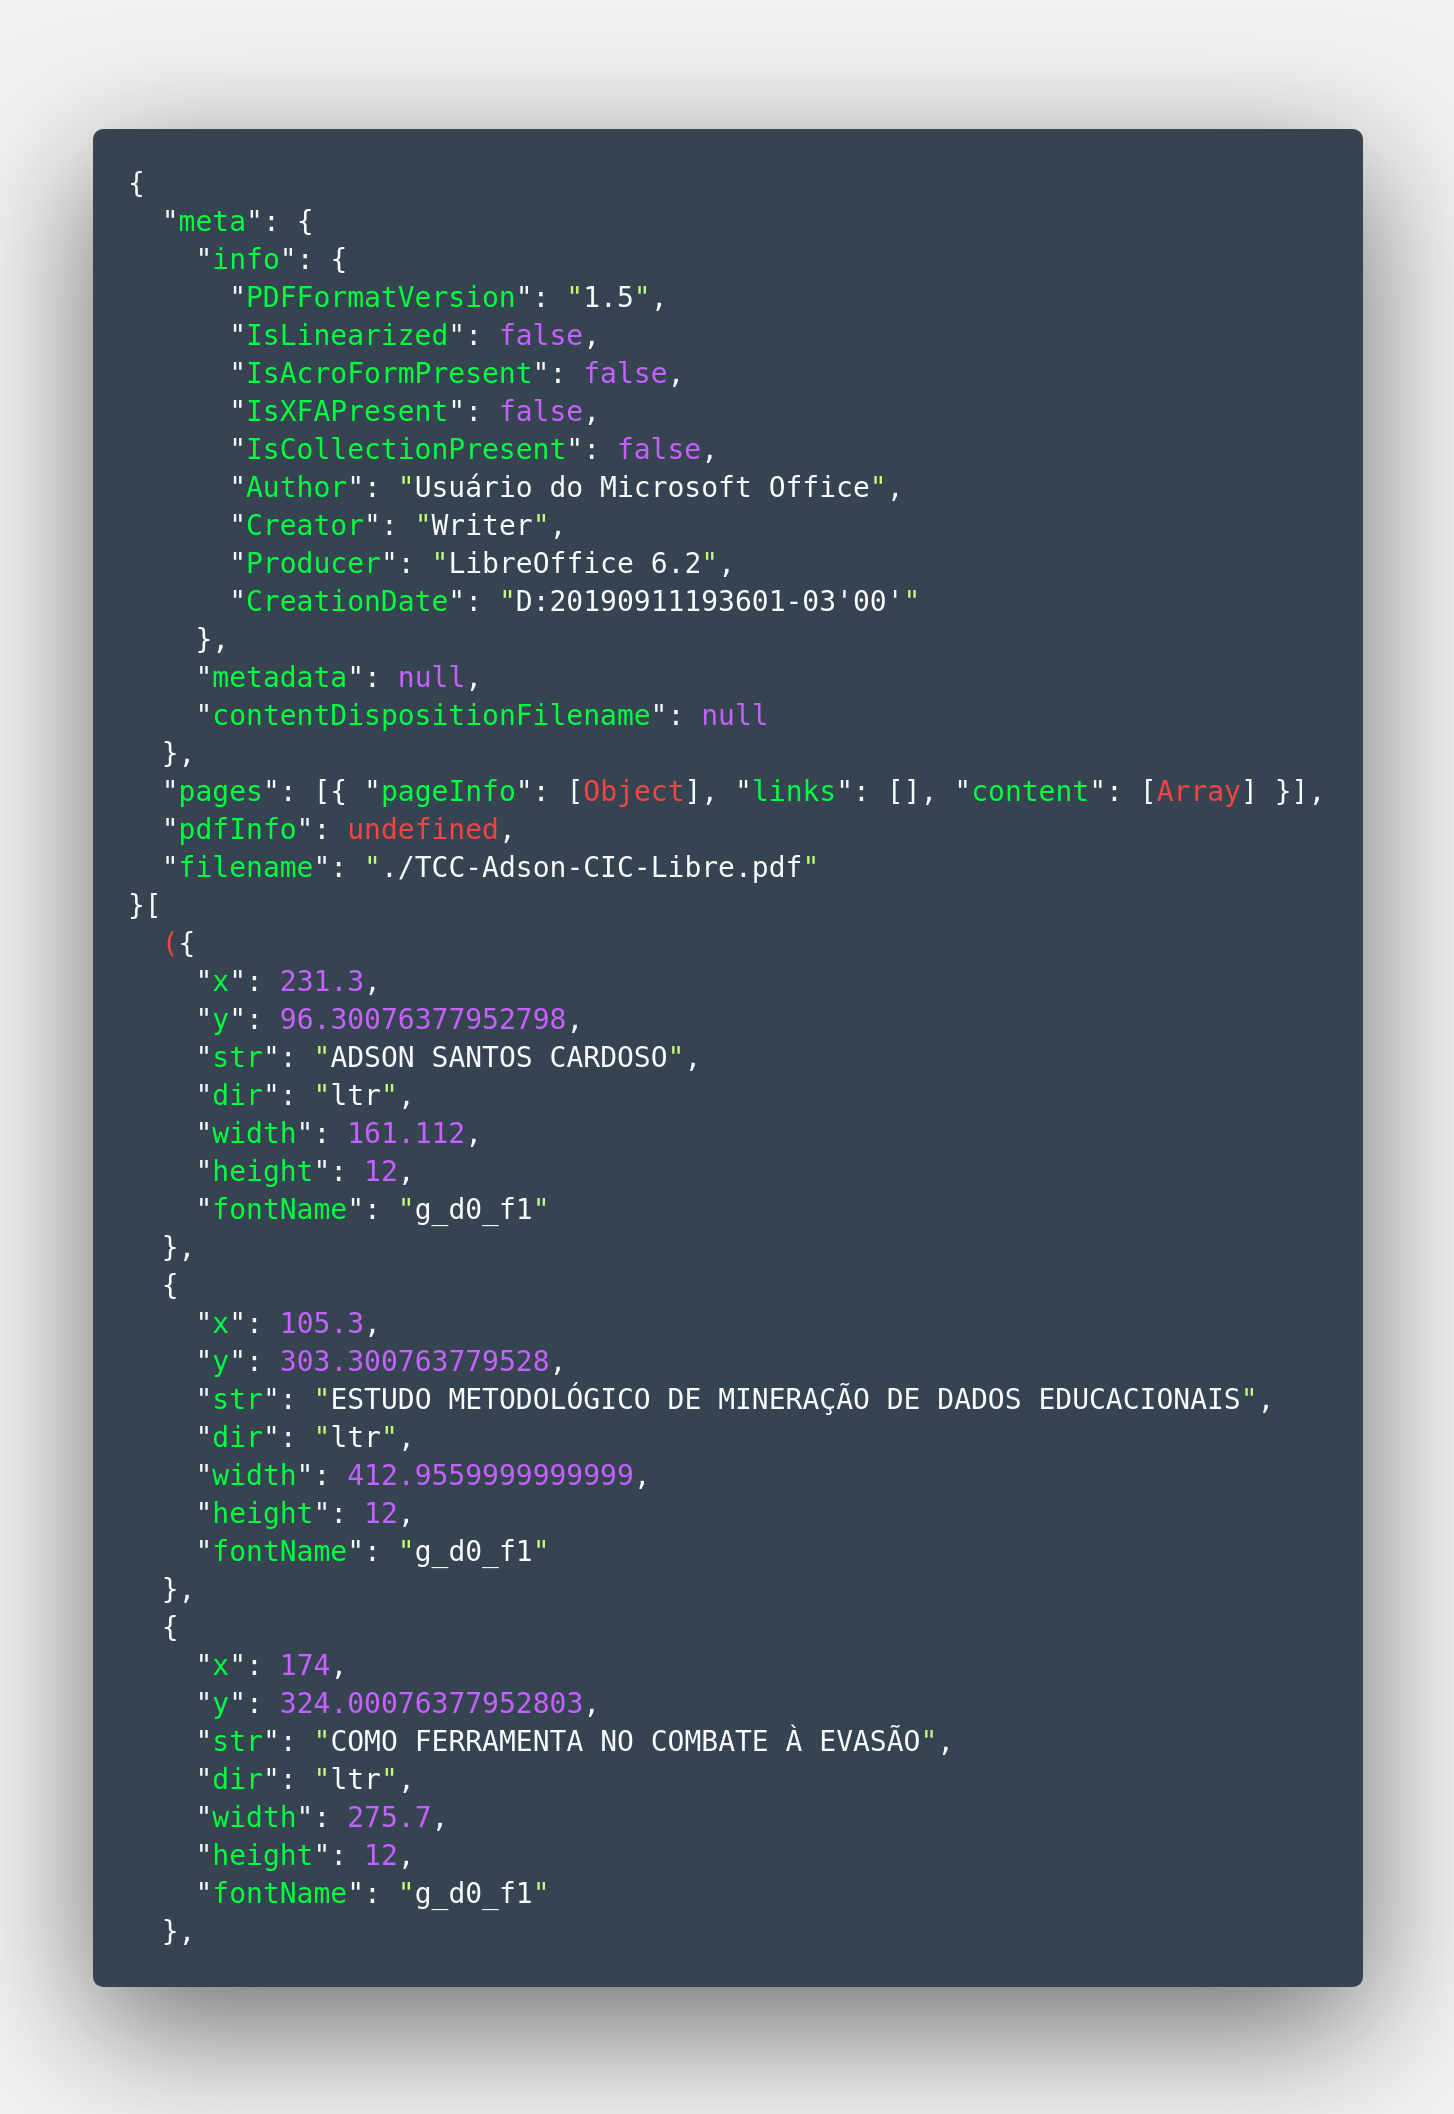
\includegraphics[scale=0.5]{figs/pdfExtract.png}
% \footnotesize Fonte: Autoria Própria
\end{figure}

Após extrair essas informações o próximo passo foi a filtragem deste conteúdo.

\subsection{Extract By Coord}

Determinado o objetivo de extrair a informação em um espaço da página que é definido por coordenadas X e Y, foi feita uma pesquisa de formas práticas para se realizar a filtragem do conteúdo, por tais coordenadas. Assim, foi encontrada uma pequena biblioteca no GitHub, com a licença MIT, que realizava uma abordagem similar à necessária para a próxima etapa da extração dos dados.

Esta biblioteca oferece duas funcionalidades: a primeira encapsula a extração feita pela biblioteca Extract, com o intuito de descartar informações desnecessárias para a análise, como a rotação, escala, tamanho da página, e evidenciar o software responsável por gerar o arquivo PDF. Além disso, os objetos na página são ordenados da esquerda a direita e de cima para baixo, e selecionado apenas os dados de coordenadas e string. Desta forma é retornado um objeto JSON enxuto, contendo apenas as informações necessárias e pronto para ser recebido como entrada da função de filtragem por área. 

Esta função é responsável por extrair o conteúdo, ela recebe o nome do programa responsável por gerar o arquivo PDF, a importância deste valor é decorrente da forma que diferentes programas atribuem diferentes formas de espaçamento entre as strings. Por exemplo o Microsoft Word realiza o espaçamento dos objetos atribuindo vários objetos de espaço, além disso são recebidos o objeto da página a ser extraída, e as coordenadas X e Y da área como objeto JSON. Ao ser executada, são observadas as coordenadas de cada objeto dentro da página, estando no alcance das coordenadas recebidas, sua string é extraída e tratada. Desta forma é retornada uma string correspondente ao conteúdo textual que se encontra naquela região.

Esta biblioteca foi alterada para que o texto recebido fosse entregue com uma formatação correta, devido a diferença de espaços causada pelo software que gerou o PDF, além disso foi feita uma melhor filtragem pelo sistema de coordenadas e a função de extração passou a aceitar mais de uma página.

\subsection{\textit{RegEx} - Expressão Regular}
% A expressão regular pode ser definida como a descrição de um padrão que identifica uma cadeia de caracteres em uma string.

O \textit{RegEx}, derivado da expressão regular definida na teoria da computação, entrega uma forma de se identificar cadeia de caracteres, dada uma expressão regular em linguagem formal. Ou seja, dada uma expressão é possível encontrar cadeias que aceitem tais condições. A linguagem JavaScript carrega todo um grupo de funções que auxiliam na utilização de expressões regulares, assim não é necessária nenhuma biblioteca adicional.

Como forma de limitação ou busca de valor específico em determinada string, são utilizadas expressões regulares que tanto removem trechos que podem afetar a busca de um valor, quanto encontram um valor específico após determinada cadeia de carácteres. Como por exemplo no caso de extração do nome de um orientador. Este nome pode se encontrar depois da palavra "Orientador" e antes da palavra 
"Coorientador", assim é definido um padrão \textit{RegEx} que encaixe com o valor que se encontra entre as duas palavras.

A filtragem com o \textit{RegEx} assegura o conteúdo encontrado e delimita a informação buscada, no caso de ocorrer um bloco inesperado dentro das coordenadas. 

\subsection{JWT - \textit{JSON Web Token} (v8.5.1) }

Com a necessidade de se ter uma forma de autenticação segura e prática, foi optado pela utilização do \textit{JSON Web Token}. Comummente, o desenvolvedor realiza a implementação de seu próprio método de autenticação, porém, segundo a \textit{Open Web Application Security Project} (OWASP), uma organização sem fins lucrativos que trabalha em prol da segurança na web, buscando falhas e formas de combater as mesmas, a “Quebra de Autenticação e Gerenciamento de Sessão” é um dos maiores e mais recorrentes problemas em aplicações web. A falta de uma boa criptografia e métodos seguros de envio e recebimento de dados ocasiona oportunidades para que usuários mal-intencionados consigam invadir contas e ter acesso a informações sigilosas.

O JWT é um padrão aberto (RFC 7519), que define de forma compacta, independente e segura, um método de transmitir informações como objeto JSON. Sendo uma forma segura, com bibliotecas para a maioria das linguagens utilizadas na web e suporte nativo do JSON nos navegadores modernos,  o JWT se tornou a escolha ideal como método de autenticação. 

Utilizando o algoritmo HMAC \textit{(Hash based Message Authentication Code)}, a informação é encriptada com um segredo que apenas o lado do servidor contém, (também podem ser utilizados pares de chave pública/privada através da encriptação por RSA ou ECDSA), e passada como um \textit{header} HTTP. Desta forma, quando o usuário realiza uma requisição que necessite de validação do usuário, o servidor recebe a \textit{header} e realiza a chamada de um método de verificação do \textit{token} contido na \textit{header} (\cite{jwt}).

\subsection{MongoDB (v4.0.13)}

O MongoDB é um banco de dados não relacional, onde os dados são armazenados em documentos JSON, por isso é dito que este é um banco orientado a documentos. Desta forma não há necessidade da criação de tabelas e colunas na fase de modelagem do banco, assim há uma liberdade maior para que o documento que será salvo represente apenas as informações necessárias e suas relações não sejam pré definidas.

Esta flexibilidade é de grande ajuda quando se trata de uma aplicação que pode mudar a organização e o tipo de informação a ser salva, diferente de um banco relacional, onde toda a sua estrutura deveria ser mudada para que se adequasse a estas mudanças. No caso dessa aplicação, o usuário irá definir quais informações serão extraídas do PDF e assim o objeto JSON com as informações será montado, além disso, o usuário também tem a liberdade de adicionar ou remover um campo de informação a ser extraída, ou adicionar um novo sem afetar a estrutura do banco.

A escolha do MongoDB entre os bancos não relacionais foi feita devido a sua alta performance, facilidade de manipulação em relação a sua infraestrutura, popularidade e principalmente a biblioteca Mongoose. 

\subsubsection{Mongoose (v5.7.5)}

A manipulação do Mongo foi feita através da biblioteca Mongoose, onde a modelagem de dados é baseada em esquemas. Ao realizar uma consulta ao banco de dados, através do mongoose, é realizada conversão do dado para um objeto JavaScript, assim quando recuperada uma informação do banco, sua manipulação se torna algo simples e orgânico no fluxo de desenvolvimento. Também é possível realizar validações através da declaração do \textit{schemas}, isso impõe mais uma camada de segurança entre o usuário e a API. 

\subsection{Express (v4.17.1)}

O Express é um \textit{framework} web baseado no modulo de \textit{http} do Node.JS, ele dispõe de vários recursos robustos e fornece muita agilidade e desempenho sem ofuscar as características do Node.JS. Além disso ele proporciona uma estrutura similar ao MVC para a organização do projeto. De forma resumida, ele entrega maneira práticas de lidar com a comunicação da aplicação com a web e fornece a possibilidade de adicionar diversos \textit{middlewares} a nível de aplicação. Algumas das principais funcionalidades oferecidas são (\cite{mardan2014express}):

\begin{itemize}
    \item Processamento de requisições HTTP;
    \item Processamento de \textit{cookies};
    \item Controle de sessão;
    \item Organizar rotas, de acordo com a URL e o método HTTP utilizado;
    \item Determinar o \textit{header} de resposta apropriado a cada tipo de dado.
\end{itemize}

\subsection{\textit{Multer} (v1.4.2)}

O \textit{Multer} é um \textit{middleware} de rota que é responsável por lidar com requisições POST do tipo \textit{multipart/form-data}, este tipo de requisição é utilizado para o envio de arquivos. Quando presente em uma rota POST, ele irá observar se é do tipo \textit{multipart/form-data}, caso não seja, a requisição será ignorada. São definidas algumas configurações para lidar com o arquivo a ser recebido, como destino do arquivo, nome, tamanho máximo e mínimo, tipo de arquivo que deve ser aceito. Desta forma ele foi utilizado para receber os arquivos PDF.

\subsection{\textit{Swagger-JS} (v3.4.0) e \textit{Swagger-UI} (v4.1.2)}

O \textit{Swagger} é um conjunto de ferramentas, construídos em torno da especificação do \textit{OpenAPI}. A organização \textit{OpenAPI} define um padrão de descrição para API's de forma que tanto humanos quanto máquinas consigam compreender e utilizar todas suas funcionalidades sem necessidade de acessar o código fonte (\citeauthor{openapi2017openapi}, \citeyear{openapi2017openapi}). 

O \textit{Swagger-JS} é uma biblioteca, que por meio de anotações no código fonte, gera uma documentação onde podem ser definidas entidades, formato de requisições, definição de rotas, respostas esperadas de determinada rota e todo tipo de capacidade da API. 

Uma das ferramentas do Swagger é o \textit{Swagger-UI}, este adiciona uma rota a aplicação onde estará disponível uma interface possuindo toda a documentação, como representado na \textbf{Figura \ref{swaggerHome}}, definida através das anotações citadas e juntamente é fornecido a possibilidade de realizar requisições diretamente desta interface como pode ser visualizado na \textbf{Figura \ref{swaggerRequest}} e consultar os dados dos modelos definidos no banco de dados como apresentado na \textbf{Figura \ref{swaggerModels}}.

\begin{figure}[H]
\centering
\captionsetup{justification   = raggedright,
              singlelinecheck = false}
\caption{Página Inicial - Swagger UI.}\label{swaggerHome}
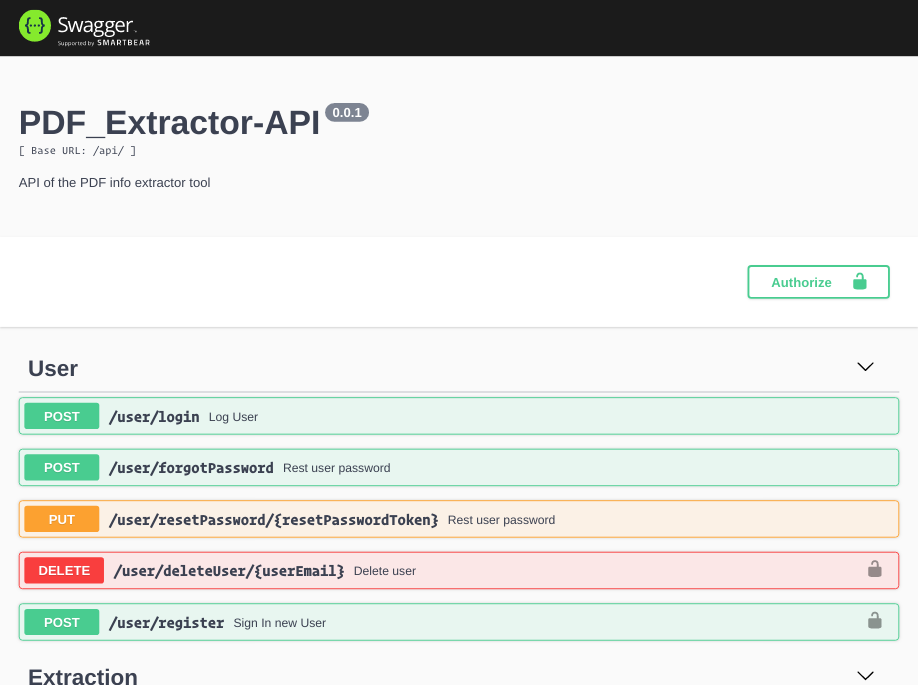
\includegraphics[width=1\textwidth]{figs/SwaggerUIHome.png}
\footnotesize Fonte: Autoria Própria
\end{figure}

\begin{figure}[H]
\centering
\captionsetup{justification   = raggedright,
              singlelinecheck = false}
\caption{Exemplo de Requisição - Swagger UI.}\label{swaggerRequest}
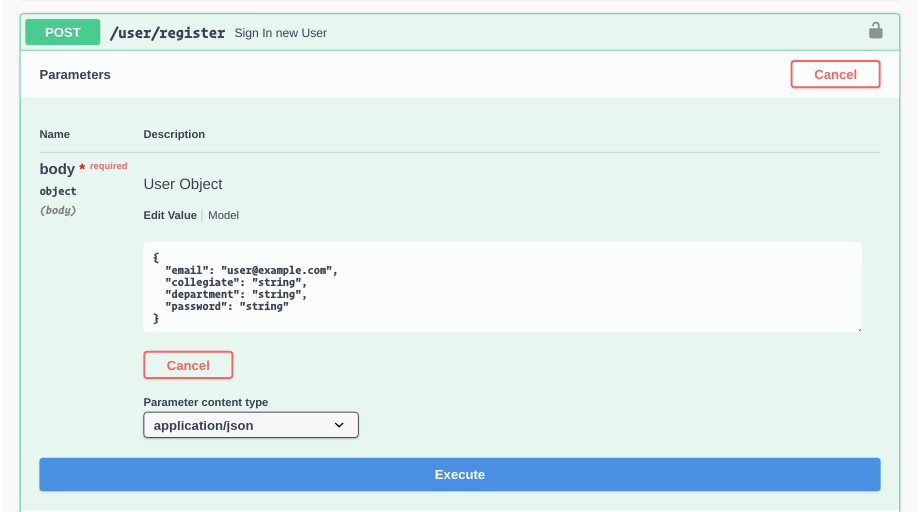
\includegraphics[width=1\textwidth]{figs/SwaggerUIExample.png}
\footnotesize Fonte: Autoria Própria
\end{figure}

\begin{figure}[H]
\centering
\captionsetup{justification   = raggedright,
              singlelinecheck = false}
\caption{Exemplo de Requisição - Swagger UI.}\label{swaggerModels}
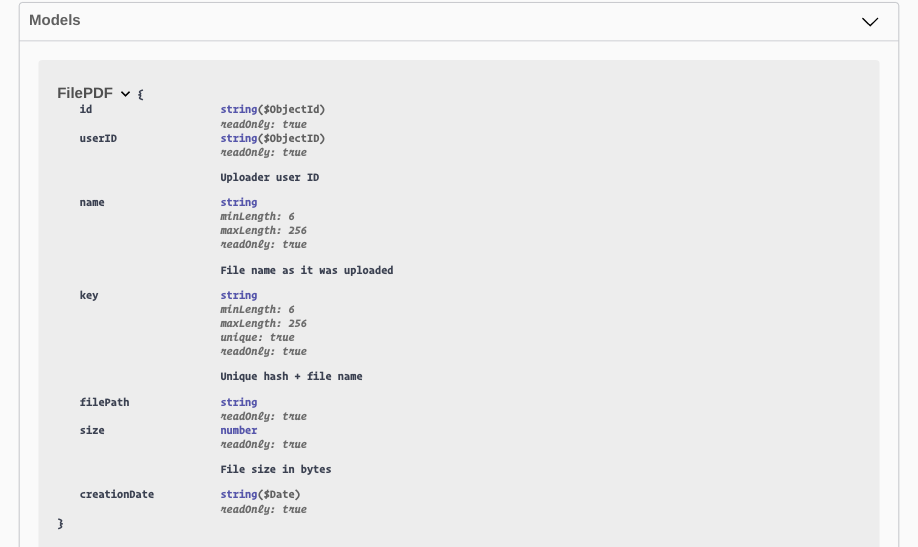
\includegraphics[width=1\textwidth]{figs/SwaggerUIModels2.png}
\footnotesize Fonte: Autoria Própria
\end{figure}


\section{Metodologia e Desenvolvimento}

Neste tópico, serão explicados como cada ferramenta foi utilizada. Os detalhes mais específicos podem ser encontrados no repositório deste projeto no GitHub, publicamente aberto e é possível enviar mudanças para que sejam avaliadas e incorporadas no código. Também será descrito como foi modelada a estrutura deste sistema e dividia as etapas de desenvolvimento.

\subsection{Kanban}

Para a organização e definição das tarefas que objetivam a completude deste projeto foi escolhida a metodologia ágil Kaban. Criado pela Toyota nos anos 70, o Kanban (que pode ser traduzido como Cartão),  sinalizava a disponibilidade para se trabalhar em uma peça, quando se fazia necessário para outras etapas da produção. Dessa forma havia uma maior organização na ordem de trabalho, não havia desperdício de peças e através dos cartões era possível ver o progresso geral.

Com estas vantagens é possível utilizar o Kanban no desenvolvimento de software e assim trazer mais vantagens ao fluxo de trabalho para a programação. 
Aplicando esta metodologia é feito um quadro consistente de três colunas, uma de tarefas \textbf{A fazer}, em seguida as tarefas \textbf{Em andamento} e finalizando com as tarefas \textbf{Concluídas}.

O GitHub oferece uma implementação do Kanban, diretamente no repositório para que outros colaboradores possam interagir e a visualização e utilização sejam práticas.

Foram separados por ordem de prioridade as tarefas necessárias para atingir a completude da API, e adicionadas nas lista de A fazer no \textit{kanban}, foram priorizadas aquelas que eram necessárias para o funcionamento e teste da API, assim foi feito uma por vez até que houvessem mais tarefas que impedissem o funcionamento de tal.

\subsection{MVC - \textit{Model View Controller}}

A estrutura deste sistema foi elaborada se baseando no padrão MVC, que tem como objetivo separar a modelagem do banco de dados, a interface do usuário e o controlador dos dados. Se baseando neste padrão foi adicionada mais uma camada chamada \textit{services}, assim é obtido mais um nível de abstração. Na \textbf{Figura \ref{MVCadptFromPressman}} é possível ver uma representação clássica do MVC e na \textbf{Figura \ref{MVSC}} a representação utilizada neste projeto.

\begin{figure}[!ht]
\centering
\captionsetup{justification   = raggedright,
              singlelinecheck = false}
\caption{Exemplo de Requisição - Swagger UI.}\label{MVCadptFromPressman}
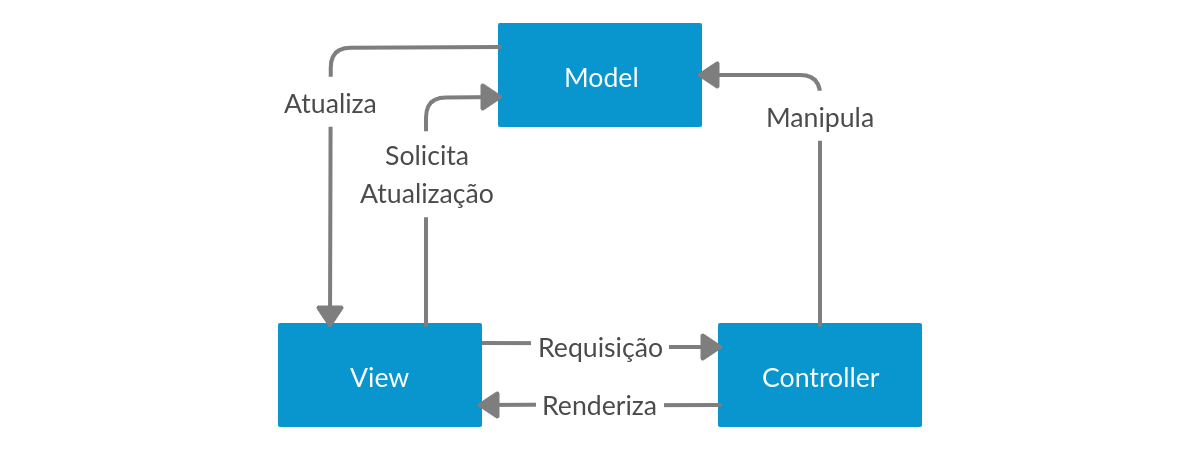
\includegraphics[scale=0.4]{figs/MVC.png}
\footnotesize Fonte: \cite{pressman2005software}, Adaptado pelo Autor
\end{figure}

\begin{figure}[!ht]
\centering
\captionsetup{justification   = raggedright,
              singlelinecheck = false}
\caption{Exemplo de Requisição - Swagger UI.}\label{MVSC}
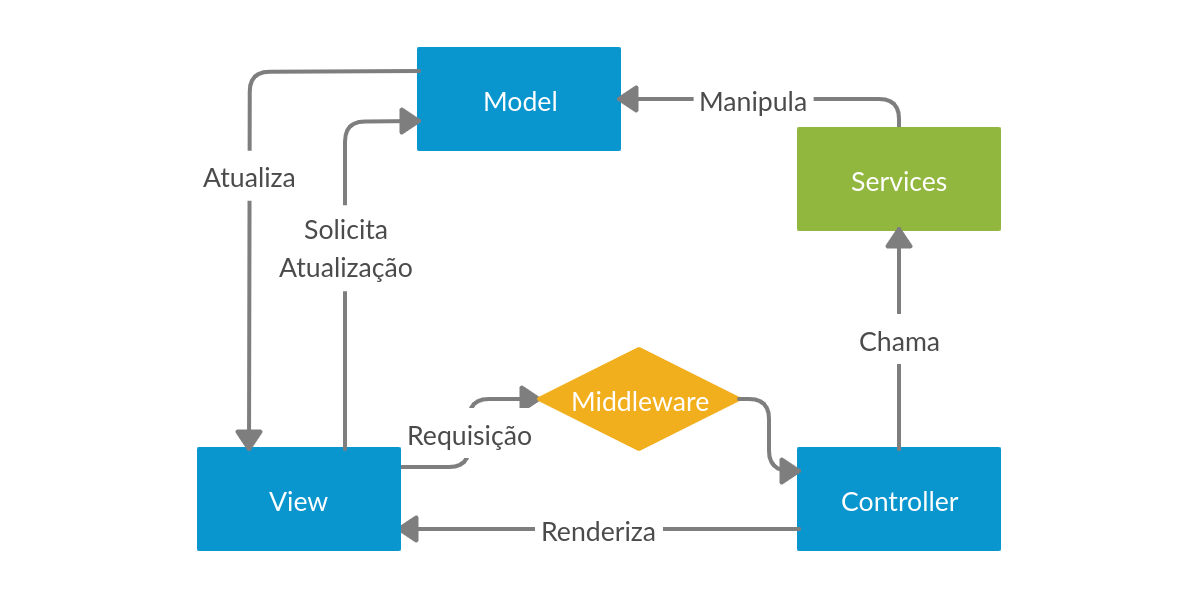
\includegraphics[scale=0.4]{figs/MVSC.png}
\footnotesize Fonte: Autoria Própria
\end{figure}

O objetivo desta camada é retirar as regras de negócio do \textit{controller}. Desta forma, o \textit{controller} possuirá apenas a responsabilidade de administrar o fluxo de dados e indicar qual o \textit{service} que deve lidar com a requisição. Dentro desta camada estão concentradas as funções que devem possuir apenas uma única responsabilidade, e ocorrendo a necessidade de uma ação complexa deve ser feita uma função responsável por chamar funções menores.

Duas principais consequências são alcançadas com esta abstração, a primeira é o baixo acoplamento, já que a lógica de negócio não está mais presente no \textit{controller} e sim uma referência a função que irá executar essa lógica. Caso haja necessidade de modificar algo na lógica, só será necessária modificar a função em questão, ou seja, não há dependência de tal para com o resto do sistema. A segunda consequência é a coesão, na camada de \textit{services} é feita uma divisão por componentes, cada componente tem uma responsabilidade específica na regra de negócios, e em cada componente estão divididas funções com apenas uma única responsabilidade.

Neste projeto foram desenvolvidos seis componentes no módulo de \textit{services}, a seguir serão apresentados estes módulos e suas finalidades:

\begin{enumerate}
    \item \textbf{\textit{authTokenService}} -
    Possui as responsabilidades de atribuir um \textit{JSON Web Token} ao usuário no momento de \textit{login}, e verificar se o \textit{token} é valido ao realizar requisições que necessitem de autenticação;
    
    \item \textbf{\textit{cryptService}} -
    Similar ao \textit{authTokenService}, porém possuindo as responsabilidades de realizar o \textit{hash} da senha do usuário e a verificação se determinada senha é válida para aquele usuário;
    
    \item \textbf{\textit{extractService}} -
    Aqui estão as funções que realizam a extração de dados. Dado o arquivo e o conjunto de parâmetros para a extração dos dados, são aplicadas as devidas configurações, provenientes destes parâmetros, e então são extraídos os dados e montado um objeto JSON com os resultados;
    
    \item \textbf{\textit{mailService}} -
    Este \textit{service} tem a única finalidade de enviar o email de recuperação de senha, ao usuário, quando solicitado;
    
    \item \textbf{\textit{filesServices}} -
    Neste \textit{service} é feito o recebimento do arquivo, proveniente do usuário, coletado dados como nome, tamanho, usuário que realizou o envio, e então renomeado com um \textit{hash} para que não ocorra problemas com duplicação;
    
    \item \textbf{\textit{userService}} -
    Aqui estão concentradas várias funções relacionadas ao usuário, sendo elas cadastro, acesso, gerar token para criação de nova senha, criar nova senha e desabilitar usuário.
\end{enumerate}
    
\subsection{Desenvolvimento da API} \label{apiDev}

Nesta seção será abordado como foi realizado o desenvolvimento da API desde o começo com o estudo das ferramentas, escolhas, modificações e como as ferramentas foram aplicadas no desenvolvimento do código. Na \textbf{Figura \ref{org}} pode ser visualizada as etapas realizadas para a conclusão da API.

\begin{figure}[H]
\centering
\captionsetup{justification   = raggedright,
              singlelinecheck = false}
\caption{Organograma das etapas de desenvolvimento.}\label{org}
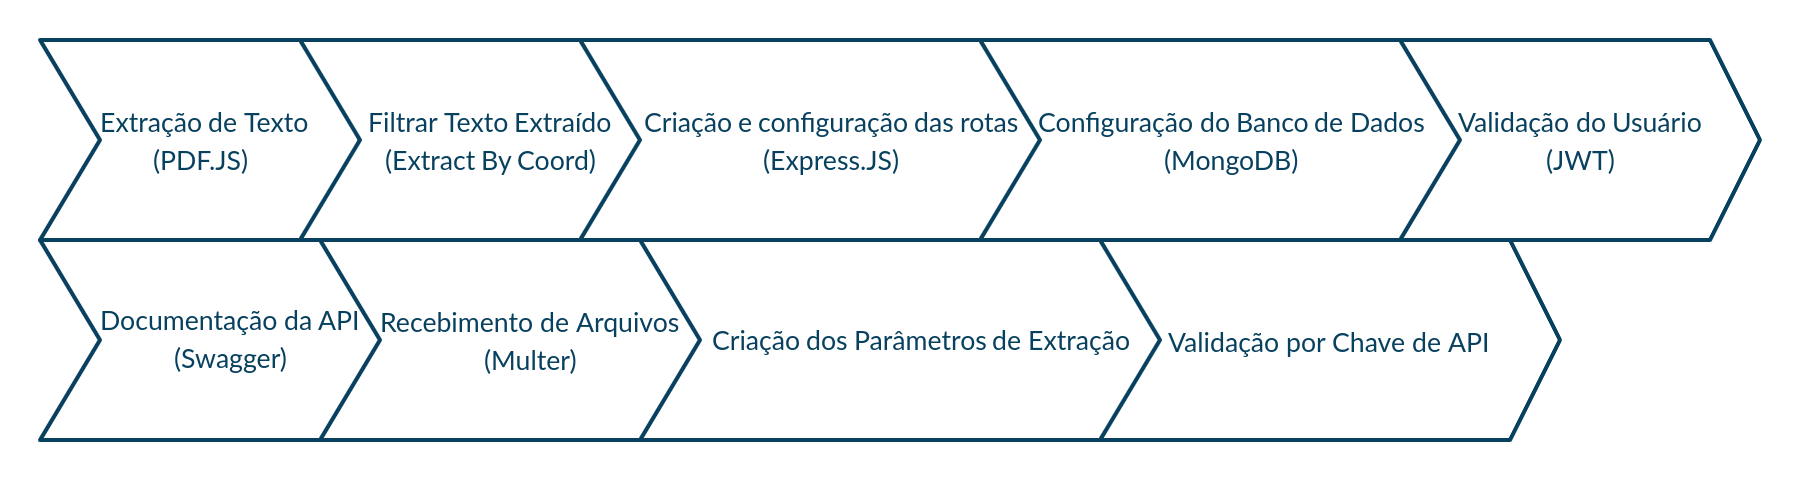
\includegraphics[width=1\textwidth]{figs/organograma.png}
\footnotesize Fonte: Autoria Própria
\end{figure}

Após definido os objetivos e o que precisava ser feito para alcança-los. Foi realizado o estudo para definir qual plataforma/linguagem seria utilizada. Conforme apontado os benefícios anteriormente, foi escolhido o Node.JS, levando em conta também a habilidade do desenvolvedor.

Tendo escolhido o Node.JS, foi necessário buscar ferramentas compatíveis com o mesmo. A primeira ferramenta estudada foi o PDF.JS, pois para viabilizar o projeto deveria haver uma forma rápida e confiável para a extração dos dados. Muitas outras bibliotecas com este mesmo objetivo foram encontradas e testadas. Porém através destes testes foi definido que o PDF.JS realizava a extração que mais se aproximava do desejado.
Havendo aspectos da extração que necessitavam melhora, foi encontrado a biblioteca que encapsulava funções do PDF.JS, o Extract. Como o PDF.JS foi criado com o foco de remontar o arquivo PDF em HTML e CSS para visualização no navegador, esta biblioteca possuía uma carga desnecessária e trazia algumas ferramentas irrelevantes ao tipo de extração em questão.

Provada a viabilidade e funcionamento da extração, foi inciada a etapa de filtragem (até então era extraído todo o conteúdo da página). Como discutido anteriormente, o tipo de filtragem que melhor funcionaria para a extração de qualquer tipo de documento PDF seria orientada a localização. Dado que o foco da extração em massa é ser guiado pela formatação da página.
A extração até esta parte continha muitos dados e nenhum tipo de filtragem, então através de pesquisas no NPM foi encontrada uma biblioteca que realizava a extração utilizando coordenadas da área desejada e retornava o conteúdo que se encontrava ali.
Contudo, devido aos diferentes softwares que realizam a montagem do PDF, o texto encontrado continha espaços e quebras de linha indesejadas e que não condiziam com o que era visualizado no documento. 

A partir daí foi iniciada a modificação a biblioteca Extract. Foram analisados os métodos de montagem utilizados pelos softwares mais populares e, definidos os casos onde ocorria o erro de formatação. Então foi desenvolvida uma função que realizava o tratamento do conteúdo, dado o software utilizado na montagem do arquivo. Além disso foi necessário adaptar a função responsável por receber o objeto dá página do PDF para que também funcionasse com mais de uma página.

A próxima etapa foi fundamentada na criação e configuração das rotas, o estudo para a decisão de qual framework seria utilizado nesta etapa foi simples, tendo em vista que o ExpressJS é o framework mais baixado no NPM (\cite{npm}) e com mais visibilidade no GitHub. A partir daí, ao comparar seus benefícios com outros frameworks ficou claro que esta seria a melhor escolha.
Decidido que a próxima etapa seria a criação do CRUD de usuário, veio a necessidade do banco de dados. 

Como dito previamente, um banco noSQL se adéqua melhor a necessidade do sistema, considerando seu crescimento e a necessidade de uma coleção livre de esquemas. Pois o conteúdo extraído será definido pelo usuário. Dentre os bancos noSQL, o MongoDB se destacou em performance e sua organização dos dados em objetos JSON se encaixou perfeitamente com as necessidades. 

Havendo a validação do usuário, se fez necessário encontrar uma forma de garantir que o mesmo estava autenticado no sistema, e para isso foi feito o estudo de tecnologias de validação. Similar ao caso do ExpressJS, foi encontrado uma tecnologia que se destacava de suas concorrentes, o JWT. Desta forma, o usuário ao se logar no sistema recebe uma \textit{header}  contendo um \textit{token} único e criptografado. E para que ele possa realizar certas requisições ele deve possuir um \textit{token} válido.

Acompanhando o crescimento da API, foi necessário iniciar o processo de documentação. Procurando fugir do moroso método clássico de documentar apenas descrevendo cada funcionalidade e suas propriedades, foi buscada uma ferramenta para que isso fosse feito de forma mais rápida e obtendo um melhor resultado.
Assim foi encontrado \textit{framework} de documentação Swagger. Este contém uma grande base de usuários e adotado por grandes empresas como a Microsoft e a National Geographic. Além de disponibilizar as funcionalidades da API para que humanos possam ler e testar, também disponibiliza de uma interface para outras aplicações que sigam o padrão estabelecido pela The Linux Foundation.

Desta forma, a utilização da API durante o desenvolvimento, foi feita utilizando a página fornecida pelo Swagger, em vista da sua facilidade e documentação apresentada.

O próximo passo foi poder receber um arquivo através de um requisição da API, e novamente, estudando tecnologias atuais, e bem utilizadas, foi encontrado o Multer. Com uma configuração simples, este \textit{middleware} foi adicionado a uma rota específica para o recebimento de arquivos, e todo o auxílio necessário para o registro deste arquivo no servidor foi feito com sucesso. Todos os cuidados como, definir o tipo de arquivo que deve ser recebido, limite de tamanho, renomear para que não haja duplicatas, foram feitos nesta configuração do Multer. Então o arquivo é recebido, se dentro da conformidade ele é aceito, renomeado com um \textit{hash} na frente, e todas suas informações são armazenadas no banco de dados.

Como o intuito é que a extração seja definida pelo usuário foi estabelecido que o mínimo que se precisa para extrair alguma informação de um documento é o número da página e as coordenadas definindo a área onde se encontra a informação. Para que o usuário possa identificar de forma prática o que foi retornado, ele deve adicionar um título, e para que ele seja capaz de filtrar o texto extraído ele pode adicionar uma \textit{RegEx}, e assim será retornado o resultado da expressão. Por fim, foi necessário acrescentar uma forma de aplicar este conjunto de parâmetros ao arquivo que o usuário deseja ter as informações extraídas. Para isso foi adicionado um campo de identificação do arquivo. Isso quer dizer que no momento de envio do arquivo, deve ser passada uma string de identificação, então será feita uma busca no banco de dados por todos os Parâmetros de Extração com esta identificação, e estes parâmetros que serão utilizados para a extração.

Assim foi desenvolvido um CRUD de Parâmetros de Extração, o objeto referente a este conta com os seguintes campos:

\begin{itemize}
    \item \textbf{\textit{extractionTitle}} - Contém o título que irá corresponder a informação extraída. 
    
    \item \textbf{\textit{page}} - Corresponde a página onde se encontra a informação desejada.
    
    \item \textbf{\textit{coordinatesStart} e \textit{coordinatesEnd}} - Coordenadas X e Y da área a ser extraída.
    
    \item \textbf{\textit{RegEx}} - Expressão regular para um filtragem mais aprimorada do trecho extraído. Este campo é opcional, caso não tenha seu valor preenchido, todo o conteúdo encontrado na área será retornado.
    
    \item \textbf{\textit{docType}} - Uma tag que será usada no momento de envio de um arquivo PDF. Ao enviar um arquivo deve ser passado um identificador, da escolha do usuário, junto a requisição. Todos os parâmetros que possuírem a tag correspondente a tal identificador serão utilizados para a extração dos dados.
\end{itemize}

Foi encontrado um obstáculo ao enviar um \textit{RegEx} à API, devido a sua formatação o valor é descaracterizado no momento que chega ao servidor e também quando salvo no banco de dados. Visando contornar este problema, foi encontrada a alternativa de codificar o valor para base64, e utilizando métodos já implementados no Node.JS, converter o mesmo para uma string e da string para um \textit{RegEx} no momento em que for utilizado.

Com o sistema sendo capaz de receber um arquivo e realizar a extração de dados em pontos específicos do documento, foi notada a necessidade de se realizar a busca de alguns dados nos casos onde a página na qual a informação se encontra não é exata. 
Assim surgiu a necessidade de uma função capaz de extrair informações de uma página não especificada. Ou seja, buscar a página e então realizar a extração. A solução encontrada consistiu em adaptar o objeto de Parâmetros de Extração para ser capaz de receber um intervalo de páginas, para que seja encontrada a página desejada o usuário deve adicionar palavras-chave que estejam contidas na página. Assim foi adicionado o campo de \textbf{\textit{keyWords}}, este campo recebe uma ou mais \textit{RegEx's}, e quando encontrada uma página que retorne resultados destas expressões, isto significa que foi encontrada a página desejada. Logo, no momento da extração dos dados, caso o parâmetro contenha um intervalo de páginas, uma função será executada, buscando neste intervalo, uma página que corresponda aos \textit{RegEx's} contidos no campo 
\textit{keyWords}. Encontrada a página, a extração da informação ocorre da mesma forma explicada anteriormente.

Para assegurar que a criação de novos usuários seja controlada, foi desenvolvido um \textit{middleware} para ser utilizado na rota de criação de usuário, o que faz obrigatório o envio de uma chave de API no momento do cadastro do usuário.

Somando as ferramentas até aqui apresentadas, e os meios encontrados para a criação desta API, foi obtido um ótimo resultado e sua empregabilidade é vasta. Tendo em vista que o estudo de tecnologias modernas não é algo simples, pode ser dito que toda escolha foi bem fundamentada e sua utilização bem descrita até o presente tópico. Conhecendo o que foi utilizado e como foi aplicado, é dado inicio aos testes e utilização da API.